%\documentclass[paper=a4, fontsize=11pt]{scrartcl}
\documentclass[11pt]{article}
\usepackage[top=1cm, bottom=1cm, left=2.5cm, right=2.5cm]{geometry}
%\usepackage[T1]{fontenc}
\usepackage{fourier}
\usepackage{float}

\usepackage[english]{babel}															% English language/hyphenation
%\usepackage[protrusion=true,expansion=true]{microtype}
\usepackage{amsmath,amsfonts,amsthm} % Math packages
\usepackage[pdftex]{graphicx}
\usepackage{url}

%%% Custom sectioning
%\usepackage{sectsty}
%\allsectionsfont{\centering \normalfont\scshape}

%%% Custom headers/footers (fancyhdr package)
%\usepackage{fancyhdr}
%\pagestyle{fancyplain}
%\fancyhead{}											% No page header
%\fancyfoot[L]{}											% Empty
%\fancyfoot[C]{}											% Empty
%\fancyfoot[R]{\thepage}									% Pagenumbering
%\renewcommand{\headrulewidth}{0pt}			% Remove header underlines
%\renewcommand{\footrulewidth}{0pt}				% Remove footer underlines
%\setlength{\headheight}{13.6pt}

%%% Equation and float numbering
\numberwithin{equation}{section}		% Equationnumbering: section.eq#
\numberwithin{figure}{section}			% Figurenumbering: section.fig#
\numberwithin{table}{section}				% Tablenumbering: section.tab#

\graphicspath{ {./images/} }

%%% Maketitle metadata
%\newcommand{\horrule}[1]{\rule{\linewidth}{#1}} 	% Horizontal rule

\title{Cache-Friendly Shuffles for Asynchronous Stochastic Optimization}

%\title{
  %\vspace{-1in}
%  \usefont{OT1}{bch}{b}{n}
%  \horrule{0.5pt} \\[0.4cm]
%  \huge Cache-Friendly Shuffles for Asynchronous Stochastic Optimization
%  \horrule{2pt} \\[0.5cm]
%}
%\author{
%  \normalfont 								\normalsize
%  \\[-3pt]
%  \normalsize
%  \today
%}
\date{}


%%% Begin document
\begin{document}

\maketitle
\section{Introduction}

In modern machine learning, many problems can be cast as instances of optimization, where the goal is to minimize some loss 
function encoding the system's errors on training data. The ubiquity of such problems has led to substantial interest in making large-scale 
optimization as efficient as possible, and a substantial portion of this work has focused on developing asynchronous algorithms that achieve 
near-ideal speedups in shared-memory systems.




\section{Least Squares}



\section{Word Embeddings}


\subsection{Problem statement}
In the word embeddings problem, given context counts $X_{w,w'}$ we want to find word vectors
$v_{w} \in \mathbb{R}^{k}$ that minimizes the loss:
\begin{align*}
\min_{v,C}\sum_{w,w'}X_{w,w'}(log(X_{w,w'}) - \|v_w+v_{w'}\|^2 - C)^2
\end{align*}

\subsection{Experimental evaluation}
\subsubsection{Methodology}

We ran our experiments on the Edison compute nodes which feature two
twelve core 2.4 GHz processors. However, we used only up to twelve
cores/threads to avoid effects of NUMA. Word vectors were length 100
double arrays.
\\\\
We used the first $10^9$ bytes of English Wikipedia from
http://mattmahoney.net/dc/textdata as corpus data. After running the text
preprocessing script supplied by the link, we computed co-occurrence
counts of pairs of distinct words to create the parameter dependence graph.
This graph was then fed into gpmetis, computing a min-k-cut partitioning to
create a cache-friendly ordering of the datapoints. k was set such that each
block of k datapoints would reference just enough word vectors to fit into the
L1-cache.
\\\\
Hogwild was then run on the permuted co-occurrence graph generated by gpmetis,
maintaining the same ordering throughout execution. Although we experimented with
both data sharding and no-data sharding, only results from data sharding are presented.
To test hogwild without a cache-friendly shuffle, we randomly shuffled the datapoints before execution.
\\\\
We also ran the experiments on subsets of the corpus, repeating the
procedure on the first $\%10$, $\%25$, $\%50$ and $\%75$ of the corpus data.
In the full corpus data, there were $~200,000$ word vectors, and $~30,000,000$
datapoints.

\subsubsection{Results}
We achieve between $\%40-\%50$ speedup over regular hogwild (non-cache-friendly hogwild),
measuring runtime to a fixed number of epochs.
\begin{figure}[H]
\begin{center}
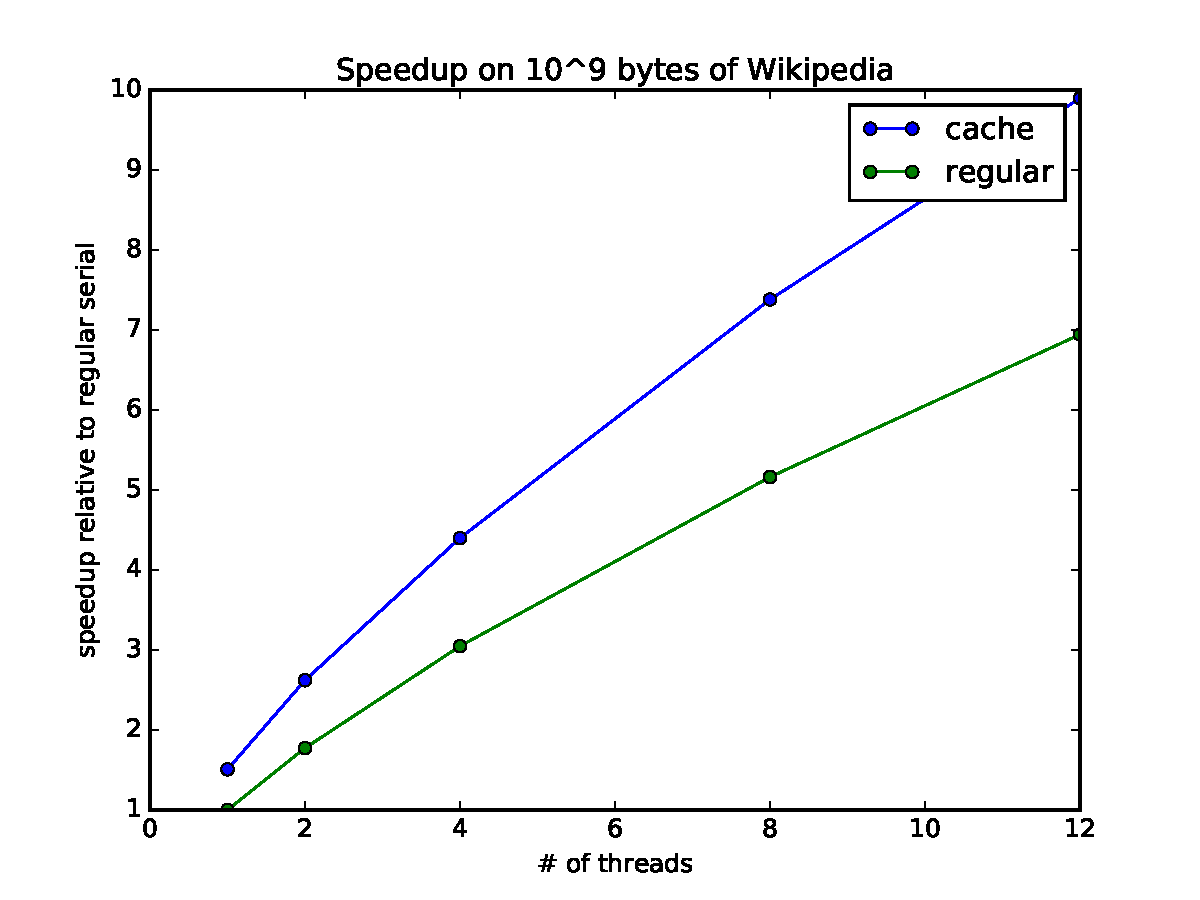
\includegraphics[width=11cm,height=11cm,keepaspectratio]{w2v_speedup_plot.pdf}
\end{center}
\end{figure}
Furthermore, the speedup is maintained on different subsets and sizes of the data.
\begin{figure}[H]
\begin{center}
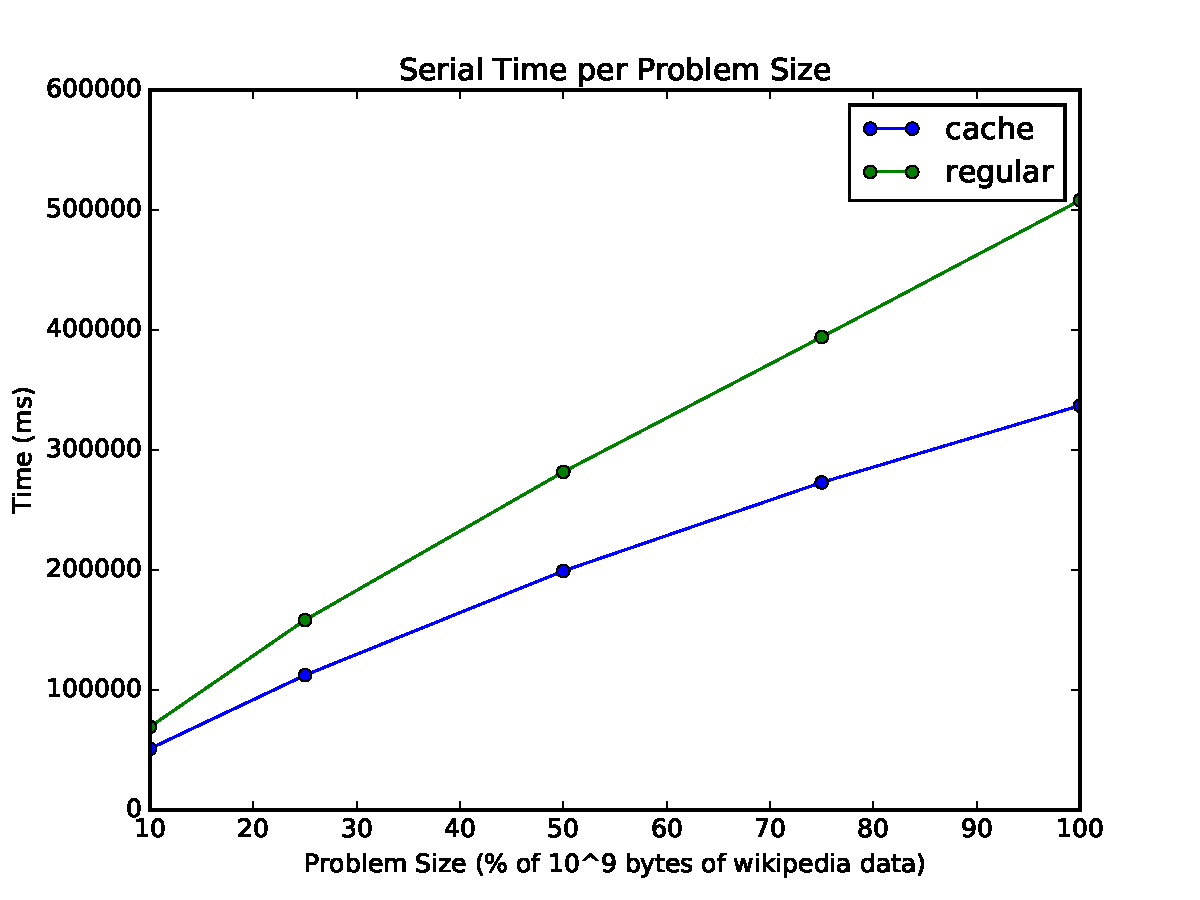
\includegraphics[width=11cm,height=11cm,keepaspectratio]{w2v_problem_size_time_plot.pdf}
\end{center}
\end{figure}
Additionally, convergence of loss is not adversely affected.
\begin{figure}[H]
\begin{center}
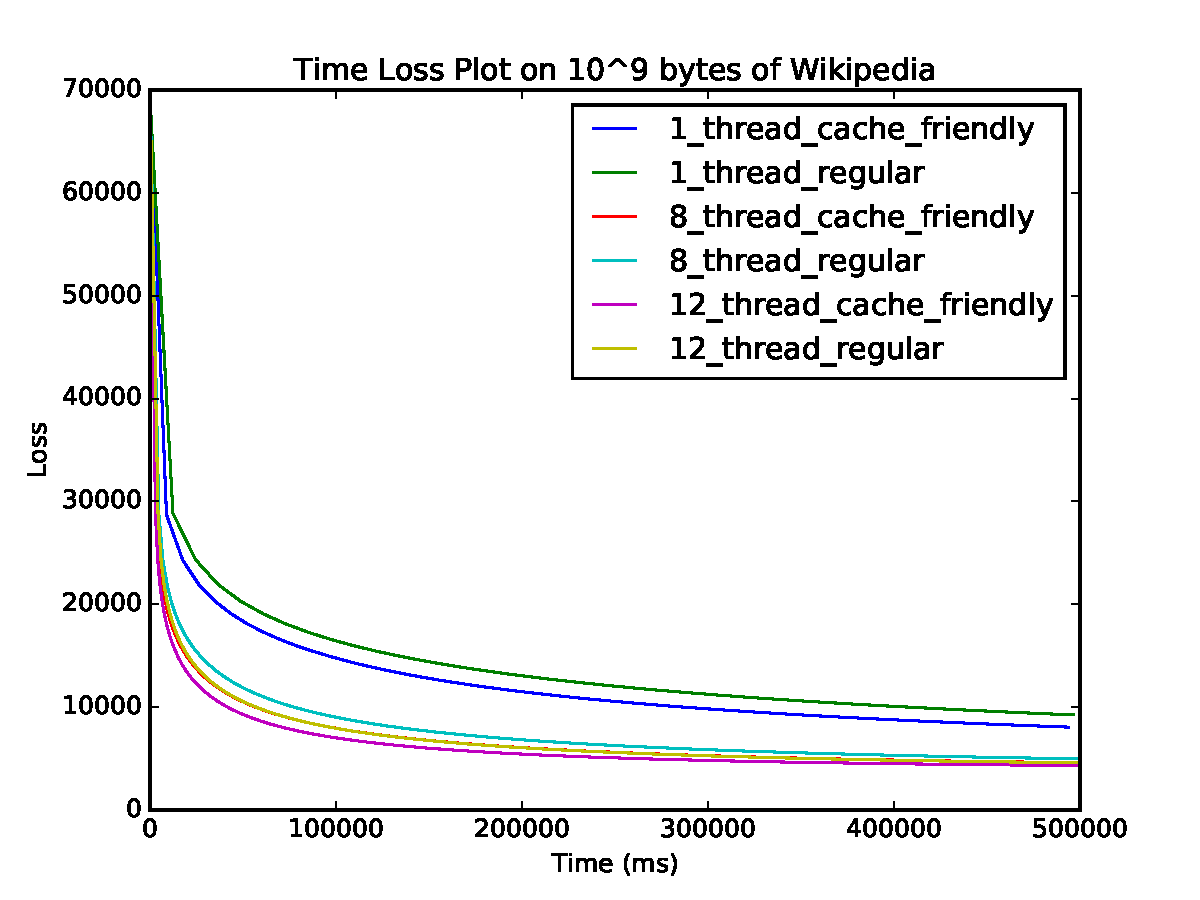
\includegraphics[width=11cm,height=11cm,keepaspectratio]{w2v_time_loss_plot.pdf}
\end{center}
\end{figure}

\subsection{Discussion}

A $\%40-\%50$ runtime gain over regular hogwild is a result of keeping
at least one length 100 double array in the L1-cache between
stochastic gradient calls. In a non-cache-friendly permutation, each
of the two vectors visited by a datapoint is typically not in the
cache, incurring two vectors worth of cache misses per
datapoint. After running min-k-cut on the parameter dependence graph,
we found that each block of k datapoints references around k distinct
vectors. Thus, in a cache-friendly permutation, one of the vectors
referenced by a datapoint is already in the L1-cache from the previous
stochastic gradient call. So a cache-friendly permutation incurs only
one vectors worth of cache misses per datapoint, naturally leading to
a $\%40-\%50$ reduction in runtime.
\newpage
\section{Conclusion}
\newpage
\section{Future}
\end{document}
